\chapter{Evaluation}
\label{chap:evaluation}
Biohadoops purpose is to facilitate the implementation of parallel algorithms on Hadoop. It is expected that the execution time of an algorithm reduces if it is parallelized (assuming the algorithm is suitable for parallelization). This chapter is devoted to the study of Biohadoops speedup characteristics.

Two bio-inspired optimization algorithms are used as benchmarks. Both use Biohadoop and its task system to solve a test problem. The algorithms and test problems are described in section \ref{chap:evaluation:testproblems}.

The algorithms are executed on a Hadoop cluster to study the impact on their execution times by varying problem sizes and number of workers. Benchmark details can be found in section \ref{chap:evaluation:benchmarks}. Results are presented in section \ref{chap:evaluation:benchmarks}.

\section{Cluster Hardware}
\label{chap:evaluation:cluster}
All experiments were performed on a Hadoop cluster with 6 identical computers. Each machine has the following specifications:

\begin{itemize}
  \item Intel Core2 Duo CPU E8200 @ \unit[2.66]{GHz} (2$\times$\unit[2.66]{GHz}, no hyperthreading)
  \item \unit[6]{MB} shared L2 cache, \unit[32]{KB} L1 data cache, \unit[32]{KB} L1 instruction cache
  \item \unit[4]{GB} (2$\times$\unit[2]{GB}) DDR2 RAM @ \unit[667]{MHz}
\end{itemize}

The computers are directly connected to the same Switch through a 1Gb (Gigabit) Ethernet network.

\section{Test Problems}
\label{chap:evaluation:testproblems}
Both implemented algorithms are part of the GA family. They differ in the number of objectives that they can handle. While NSGA-II is used to solve the MOP in section \ref{chap:evaluation:zdt3}, a simple GA is used to solve the SOP in section \ref{chap:evaluation:tiledmul}.

The benchmarks are executed on the cluster described in section \ref{chap:evaluation:cluster}. The assumption is that the execution time of an algorithm depends both on the problem size and the number of workers. To evaluate this assumption, the algorithms presented in section \ref{chap:evaluation:testproblems} are executed with different problem sizes and different numbers of workers. The execution times are measured and used to calculate the speedup using the formula $S = T_S / T_P$. Here, $S$ is the speedup, $T_S$ is the time for sequential execution of the algorithm and $T_P$ is the time for parallel execution. The sequential execution uses a single worker for the compute intensive parts. It relies on the network --- like the parallel execution --- since the worker can run anywhere in the cluster. The parallel execution uses 2 to 15 workers.

A single benchmark is defined by a given algorithm (e.g. NSGA-II) and its settings (e.g. number of workers, number of iterations, etc.). All performed benchmarks have the following settings in common:
\begin{itemize}
  \item The number of iterations is set to 250.
  \item The population size is set to 100.
  \item The distribution index $n_c$ for the SBX crossover is set to 20.
  \item The distribution index $n_m$ for the mutation is set to 20.
  \item The mutation probability for each offspring value is set to $1/n$, i.e., on average one offspring value is mutated.
\end{itemize}

Each benchmark for a given setting is repeated five times to improve the reliability of the results. The results are discussed in section \ref{chap:evaluation:result}.

% The execution time for each setting is measured for a number of workers that range from 1 (sequential) to 15 (parallel). Each benchmark is repeated five times to improve the reliability of the results, making it 300 benchmark runs for ZDT-3 (4 genome sizes $\times$ 15 worker setting $\times$ 5 repetitions) and 150 benchmark runs for TMM (2 tile sizes $\times$ 15 worker settings $\times$ 5 repetitions).

\subsection{ZDT-3}
\label{chap:evaluation:zdt3}
The first optimization algorithm is NSGA-II, used to find optimal solutions for the Zitzler–Deb–Thiele's function nr. 3 \cite{zitzler2000comparison}. ZDT-3 is part of the well known ZDT family of MOP. It was chosen because of its discontinuous Pareto Front (see figure \ref{fig:zdt3}) which can be hard to find for optimization algorithms. The expected outcome is to find an approximation to the optimal Pareto Front.

\begin{figure}
  \centering
  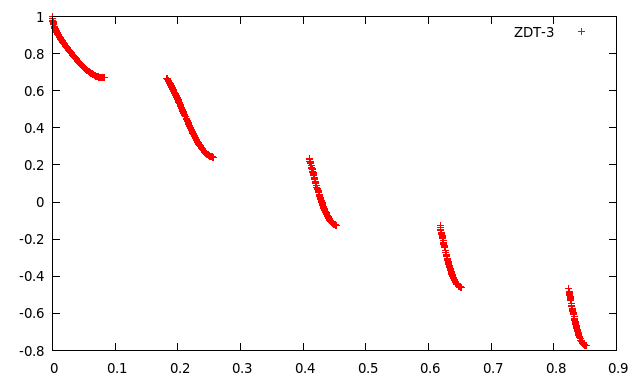
\includegraphics[width=110mm,natwidth=640,natheight=384]{zdt3.png}
  \caption[Optimal Pareto Front for ZDT-3]{Optimal Pareto Front for ZDT-3}
  \label{fig:zdt3}
\end{figure}

The ZDT-3 benchmarks are executed with genome sizes of 10, 100, 1000 and 10000, using 1 to 15 workers. Since each benchmark is repeated five times, this makes 300 benchmark runs (4 genome sizes $\times$ 15 worker settings $\times$ 5 repetitions).

The genome size corresponds to the number of values of an individual and the dimension of the solution space. Each individual is represented by its genome. ZDT-3 can handle any genome size. Changing this number influences two properties of the ZDT-3 benchmark. First, increasing the number of genomes also increases the computation effort for the workers that generate new offsprings and compute their fitness. This is due to the fact that workers generate new individuals using parent genomes and that the ZDT-3 algorithm, used for the fitness computation, loops over all genomes. Second, the genome size influences the amount of data that has to be transferred between the master and the workers. Each worker repeatedly receives two parent individuals and returns an offspring and its computed fitness. The amount of data sent between master and workers is, therefore, related to the gnome size of each individual.

The implementation uses Biohadoop workers to create and evaluate the offsprings. Simulated Binary Crossover (SBX) and Parameter based mutation \cite{deb2000efficient} are used for the offspring creation. The fitness is computed using the ZDT-3 function. The selection of the fittest individuals for the next population is based on ranking and crowding distance and is performed on the master.

\subsection{Tiled Matrix Multiplication}
\label{chap:evaluation:tiledmul}
The second benchmark implements a GA to solve the SOP for finding optimal tile sizes for the tiled matrix multiplication (TMM). The objective is to minimize the execution time for a matrix multiplication.

A matrix multiplication can be performed in different ways. The most obvious one is the standard algorithm:
\begin{lstlisting}
for i = 1 to n
  for j = 1 to m
    for k = 1 to l
      C(i,j) = C(i,j) + A(i,k) * B(k,j)
\end{lstlisting}

The matrix multiplication can be improved by loop tiling \cite{wolfe1989more}. The computation is performed on smaller blocks (tiles) of the matrices:
\begin{lstlisting}
for i0 = 1 to n, step blocksize_i
  for j0 = 1 to m, step blocksize_j
    for k0 = 1 to l, step blocksize_k
      for i = i0 to min(i0 + blocksize_i, n)
        for j = j0 to min(j0 + blocksize_j, m)
          for k = k0 to min(k0 + blocksize_k, l)
            C(i,j) = C(i,j) + A(i,k) * B(k,j)
\end{lstlisting}

If the blocks are small enough they fit into the L1 CPU cache which results in a speedup. For example, the average of ten consecutive test multiplications of two matrices of size 1024$\times$1024 took 11.384 seconds for the simple matrix multiplication and 2.669 seconds for the tiled multiplication with tile sizes $i=32$, $j=32$ and $k=32$, using a single computer of the test system mentioned above. This numbers show that it is appropriate to use the tiled approach for the matrix multiplication. But the speed of TMM depends heavily on the tile sizes, the same tiled multiplication as above with tile sizes of $i=1$, $j=1$ and $k=1$ took 25.683 seconds to finish, an increase of about 10 times compared to a good tile size. Because of the number of possible tile size combinations and the time it takes to execute a matrix multiplication (e.g. matrix size=1024, 2 seconds for a matrix multiplication: $1024^3 \times 2 = 2\times{10^9} $ seconds), it is not feasible to do an exhaustive search for the optimal tile sizes.

An optimization algorithm can be used to find the (near) optimal tile sizes for the different loops. In this case, the optimization is done using a GA. The implementation uses Biohadoops workers to create and evaluate an offspring. For the offspring creation, Simulated Binary Crossover (SBX) and Parameter based mutation are used. The fitness is computed as the time it takes to multiply two matrices using a given tile size. The selection of the fittest individuals for the next population is performed on the master.

The TMM benchmarks are executed with matrix sizes of 128$\times$128 and 256$\times$256. The matrix size influences the number of computations that need to be performed for a full matrix multiplication and, therefore, also influences the execution time. In contrast to ZDT-3, the matrix size has no impact on the amount of data transferred between the master and the workers. The matrices are part of the ``initial data'' (see chapter \ref{chap:impl:worker}) and, hence, transferred exactly once to every worker. The task data consists of two parent individuals that are transferred from the master to the workers to create a new offspring and compute its fitness. The data transferred from a worker to the master contains the offspring and its computed fitness value. Each individual consists of its tile sizes for $i$, $j$ and $k$.

\section{Results}
\label{chap:evaluation:result}
The execution time of a Biohadoop application is composed of the time Biohadoop needs to start up and the algorithm execution time. The start up begins with Biohadoops submission to Hadoop and ends when the algorithms \texttt{run} method is invoked. The algorithm execution time starts with the invocation of the algorithms \texttt{run} method and ends when this method returns.

The distinction between start up time and algorithm execution time is made because the main part of the start up time is spent between the application submission to YARN and the beginning of its execution. It is not possible to predict when an application is executed by Hadoop as it depends on different factors like the available cluster resources. To minimize the impact of this uncertainty, the benchmark measurements are based on the algorithm execution time, without the application start up time.
% . The start up time over all benchmarks range from \unit[2.378]{s} to \unit[6.147]{s}, with a median of \unit[3.864]{s}, a \unit[25]{\%} quartile of \unit[3.145]{s} and a \unit[75]{\%} quartile of \unit[4.258]{s}. The mean value is \unit[3.781]{s}. These start up times are close to each other, because the used cluster was completely dedicated to the benchmarks. The start up may take longer when the cluster usage is higher.

Lower and upper maximum speedup bounds are established to measure and compare the speedups of the benchmarks. This is done because it is difficult to compute exact maximum theoretical speedup results based on the algorithm execution time. Those times are influenced by many factors, e.g, free resources on the computers, YARN behavior, etc. The different factors are mentioned during the presentation of the results in the next sections. An overview of all recognized effects is given at the end of this chapter.

The bounds are computed using the serial execution times of the benchmarks. Since each benchmark is repeated five times it is possible to compute the lower and upper bounds from this measurements. The bounds are, although, still estimates. More benchmarks would most likely produce different bounds.

The bound computation is done using the formula $S = T / (T - t_p)$ from Amdahl's law \cite{amdahl1967validity}, where $S$ is the speedup. The serial algorithm execution time $T$ is measured using one worker and doesn't include the startup time, as explained above. The time spent in parallel code parts $t_p$ is measured on the master and comprises the time between task submission and result reception for all tasks.

Table \ref{table:speedup_bounds} shows the lower and upper speedup bounds. Immediately recognizable is the fact that the lower and upper bounds differ largely, e.g., in the case of NSGA-II with 10 genomes the difference is more than a factor of two. This is a strong hint that algorithm execution times on Hadoop depend on more factors than just the algorithm parameters. The algorithm execution time results for the benchmarks can be found in the boxplots in figures \ref{fig:nsga_250_100_10}, to \ref{fig:nsga_250_100_10000} for the ZDT-3 benchmarks and in figures \ref{fig:tiledmul_250_100_128x128} and \ref{fig:tiledmul_250_100_256x256} for the TMM. The number of workers and the algorithm execution time is plotted on the x-axis and y-axis, respectively.

\begin{table}
  \centering
  \caption{Upper and lower speedup bounds}
  \begin{tabular}{lrr}\toprule[2pt]
    Test Problem & Lower bound & Upper bound \\ \midrule
    NSGA-II, 10 genomes & 4.816 & 11.046 \\ %/sdb/studium/master-thesis/benchmarks/nsgaii/250_100_10_0.5.1-SNAPSHOT_1/application_1417688654343.out2
    NSGA-II, 100 genomes & 5.228 & 9.398 \\ % /sdb/studium/master-thesis/benchmarks/nsgaii/250_100_100_0.5.1-SNAPSHOT_1/application_1417692476922.out2
    NSGA-II, 1000 genomes & 9.438 & 20.275 \\ % /sdb/studium/master-thesis/benchmarks/nsgaii/250_100_1000_0.5.1-SNAPSHOT_1/application_1417694542512.out2
    NSGA-II, 10000 genomes & 8.861 & 17.081 \\ % /sdb/studium/master-thesis/benchmarks/nsgaii/250_100_10000_0.5.1-SNAPSHOT_1/application_1417696479026.out2
    128$\times$128 tiled mul & 63.649 & 134.404 \\ % /sdb/studium/master-thesis/benchmarks/tiledmul/250_100_128x128_0.5.1-SNAPSHOT_1/application_1417708147765.out2
    256$\times$256 tiled mul & 139.685 & 271.925 \\ \bottomrule[2pt] % /sdb/studium/master-thesis/benchmarks/tiledmul/250_100_256x256_0.5.1-SNAPSHOT_1/application_1417950505363.out2
  \end{tabular}
  \label{table:speedup_bounds}
\end{table}

% \begin{itemize}
%   \item Free resources (CPU, RAM, Network) on the machine: The utilization of a machine by other processes influences the execution times.
%   \item Network package size: The network in use has a maximum package size. If data packets exceed this size, they need to be chunked into several smaller packets.
%   \item JIT (Just-in-time compiler): the Java just-in-time compiler compiles Java byte code into machine executable code that can be executed faster. This compilation is done only if a a certain part of a Java program is called several times (typically after 10000 calls). JIT optimized code executes faster than interpreted code, but takes itself some time to get compiled
%   \item Netty and Kryo performance: Netty provides the network functionality for Biohadoop, Kryo is used for serialization. Both are executed on the master and worker processes and have influence on the algorithm execution times due their need for resources. It is hard to estimate how Netty and Kryo behave for different data sizes, e.g., kt is tunable how much buffer memory Kryo allocates by default for serialization/deserialization. 
%   \item L1 / L2 cache sharing and pollution: The CPUs used for the benchmarks have a per-core L1 cache of \unit[32]{KB} and a shared L2 cache of \unit[6]{MB}. Since several processes run on each machine (.e.g. the operating system and the Hadoop processes), it is hard to estimate how much cache is available for the benchmark execution.
%   \item YARN container placement: The benchmark algorithm execution times depend on the placement of the YARN containers.
%   \item YARN container startup time (master and worker containers): It may take arbitrary time for YARN to start a container. This can not be influenced.
%   \item Operating System (OS): The OS needs resources itself. It provides the resources for the benchmark execution and the transmission of network data. Especially the second component can have an influence on the execution times.
% \end{itemize}

% Table \ref{table:theoretical_speedup} gives an impression how well the benchmark problems are suited to parallelization by showing the maximum theoretical speedup. The theoretical speedup was calculated using the formula $S = T / (T - t_p)$ from Amdahl's law \cite{amdahl1967validity}, where $S$ is the speedup, $T$ the algorithm execution time and $t_p$ is the time spent in code parts that are parallelized using Biohadoops task system. $T$ and $t_p$ were taken from the average benchmark times with one worker.

% \begin{table}
%   \centering
%   \caption{Theoretical speedups}
%   \begin{tabular}{lr}\toprule[2pt]
%     Test Problem & Theoretical Speedup \\ \midrule
%     NSGA-II, 10 genomes & 7.028 \\
%     NSGA-II, 100 genomes & 7.600 \\
%     NSGA-II, 1000 genomes & 12.008 \\
%     NSGA-II, 10000 genomes & 11.124 \\
%     128$\times$128 tiled mul & 81.359 \\
%     256$\times$256 tiled mul & 212.169 \\ \bottomrule[2pt]
%   \end{tabular}
%   \label{table:theoretical_speedup}
% \end{table}

% One can see from the theoretical speedups that ZDT-3 is not well suited for parallelization. This is due to the fact that the fitness evaluation is not compute intense. Its time consuming part is a sum over the genomes of an individual, implemented as loop. For example, in the case of 10 genomes per individual this loop would be repeated 10 times. Bigger genome sizes mitigate this effect but have the drawback that the communication time between the master and the workers increases, which negatively affects the speedup. TMMs on the other side show a big potential for parallelization.



\subsection{Influence of YARN Container Placement}
The first thing to note when looking at the figures \ref{fig:nsga_250_100_10} to \ref{fig:tiledmul_250_100_256x256} is that the five benchmark times for a given setting (e.g. NSGA-II, 10 genomes) and one worker are very different. The explanation for this effect can be found in the YARN container placement. If a worker container is executed on the same machine as the master container, they communicate without using the physical network. This effect brings a huge performance gain, as can be seen for example in figure \ref{fig:nsga_250_100_100}. In the single worker benchmarks, 4 out of 5 benchmarks executed with both the master and worker container running on the same machine. The result was a \unit[50]{\%} better performance (\unit[9.761]{s} average) compared to the fifth benchmark (\unit[14.164]{s}) where the master and worker were executed on different machines. Potential research projects could focus on a Hadoop scheduler that tries to put a YARN ApplicationMaster and its containers on the same machine to reliably produce similar results.

The number of worker containers running on the same machine as the master can also have a negative effect on the execution times. This is especially true if the master is already at the limit of the machines resources and must share them with the workers. An example for this can be found in figure \ref{fig:nsga_250_100_10} for 8 workers. Two worker containers were executed on the same machine as the master during 2 out of 5 benchmarks. The execution time results were \unit[87.977]{s} and \unit[88.014]{s}. In the remaining 3 benchmarks, only one worker container was executed on the same machine as the master, leaving more resources to the master. This results in execution times of \unit[68.423]{s} on average, a difference of more than \unit[20]{\%}.

Therefore, it depends on the available resources of a machine if the execution of worker containers on the same machine as the master container provides benefits or drawbacks. If a resource like CPU or network is already at its limit, additional worker containers slow the whole Biohadoop execution down. If there are enough resources available, the execution of worker containers on the same machine as the master provides benefits, as the communication between the master and the workers can be performed without network usage.

The location of the YARN containers can currently not be influenced, but discussions by the YARN developers suggest that future versions of YARN will support this feature.

% \subsection{CPU Influence}
% The CPU has big influence on the algorithm execution times. If the CPU u
% 
% \subsection{RAM Influence}
% All benchmarks start with \unit[256]{MB} of Java heap memory, which is enough for the containers to execute without causing excessive garbage collections. This was established by using the tool jvisualvm (delivered with Java) for the ZDT-3 benchmark with 10000 genomes and the TMM with a matrix size of 256x256. The memory usage for the master container is at about \unit[100]{MB} to \unit[150]{MB}. The activity of Java's garbage collector at the master takes about \unit[5]{\%} of the CPU time. This value would be significantly higher in case of a memory problem. The memory usage for a worker is even lower and lies in the range of \unit[5]{MB} to \unit[30]{MB}. Again, this numbers show no significant memory problems.

\subsection{ZDT-3}
\label{chap:evaluation:result:zdt3}
The next thing to notice are the speedups for the ZDT-3 benchmarks. ZDT-3 is not well suited for parallelization as can be seen from the speedups in table \ref{table:speedup_bounds}, but the results are even worse than expected, with maximum speedups of 1.619 for 10 genomes, 1.513 for 100 genomes, 2.498 for 1000 and 2.479 for 10000 genomes. Figure \ref{fig:speedup} shows the speedup results of the ZDT-3 benchmarks together with the speedups for TMM.

\begin{figure}
  \centering
  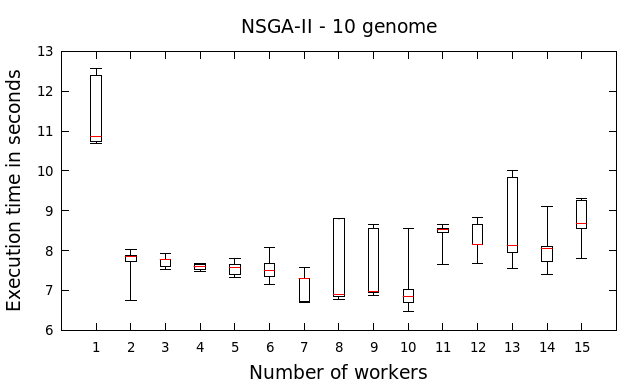
\includegraphics[width=100mm,natwidth=640,natheight=384]{nsgaii_250_100_10.png}
  \caption[ZDT-3 execution times for a genome size of 10]{ZDT-3 execution times for a genome size of 10}
  \label{fig:nsga_250_100_10}
\end{figure}
\begin{figure}
  \centering
  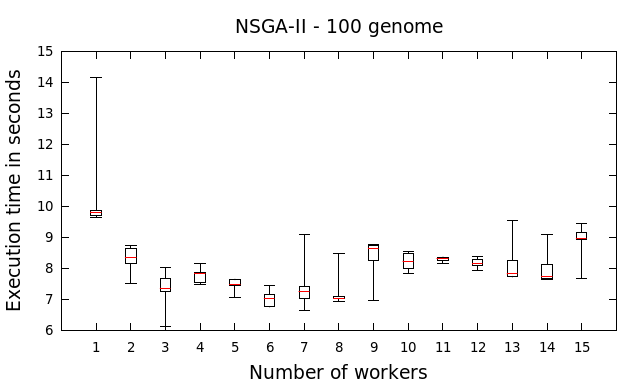
\includegraphics[width=100mm,natwidth=640,natheight=384]{nsgaii_250_100_100.png}
  \caption[ZDT-3 execution times for a genome size of 100]{ZDT-3 execution times for a genome size of 100}
  \label{fig:nsga_250_100_100}
\end{figure}
\begin{figure}
  \centering
  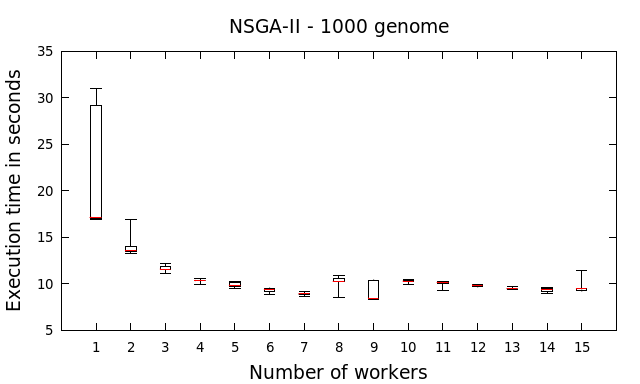
\includegraphics[width=100mm,natwidth=640,natheight=384]{nsgaii_250_100_1000.png}
  \caption[ZDT-3 execution times for a genome size of 1000]{ZDT-3 execution times for a genome size of 1000}
  \label{fig:nsga_250_100_1000}
\end{figure}
\begin{figure}
  \centering
  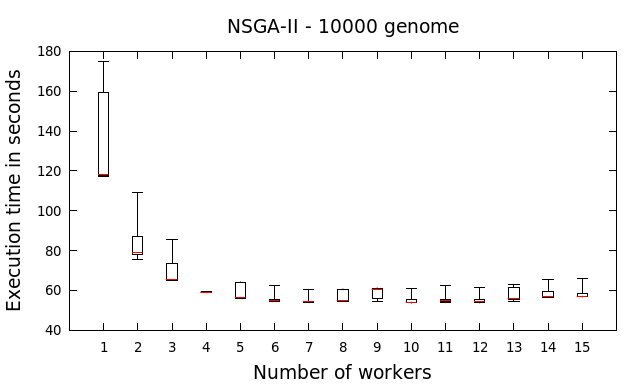
\includegraphics[width=100mm,natwidth=640,natheight=384]{nsgaii_250_100_10000.png}
  \caption[ZDT-3 execution times for a genome size of 10000]{ZDT-3 execution times for a genome size of 10000}
  \label{fig:nsga_250_100_10000}
\end{figure}

The ZDT-3 benchmarks seem to suffer from the lack of one or more resources (bound by the resources), which prohibits further speedup increases. The investigations show that the ZDT-3 benchmarks are not bound by memory, i.e., memory issues don't slow the execution down. All benchmarks start with \unit[256]{MB} of Java heap memory, which is enough for the containers to execute without causing excessive garbage collections. This was established by using the tool jvisualvm (delivered with Java) for the ZDT-3 benchmark with 10000 genomes. The memory usage for the master container is at about \unit[100]{MB} to \unit[150]{MB}. The activity of Java's garbage collector, a good indicator for memory problems, ranges from \unit[3]{\%} to \unit[5.5]{\%} of the CPU time, with an average of \unit[3.8]{\%}. The memory usage for a worker is even lower and lies in the range of \unit[5]{MB} to \unit[30]{MB}. This numbers show no significant memory problems.

% So it must be clarified if the ZDT-3 benchmarks are network or CPU bound. Figures \ref{fig:nsgaii-workertime} and \ref{fig:nsgaii-tasktime} provide some helpful data. Figure \ref{fig:nsgaii-workertime} depicts the mean time spent by the workers in the \texttt{compute} method for a single task. The figure shows that the worker times scale with the number of workers. The maximum scale factor is 4.235 for 10 genomes, 8.571 for 100 genomes, 10.744 for 1000 genomes and 11.923 for 10000 genomes.
% 
% Unfortunately no provable explanation was found why small genome sizes scale worse on the workers, compared to bigger genome sizes. A possible reason is Javas JIT (just in time) compiler that compiles interpreted Java code to machine code, thus providing better performance for the future executions. JIT is applied to code parts that are invoked more than 10000 times. This limit is reached late for small genome sizes. For example, the code of the ZDT-3 loop is compiled only after 1000 tasks in the 10 genome benchmarks. In contrast, the loop compilation is performed already after the first task for a genome size of 10000.
% 
% Increasing the number of workers worsens the problem as it decreases the amount of work performed by each worker, but as already mentioned, this explanation could not be no proved.
% 
% \begin{figure}
%   \centering
%   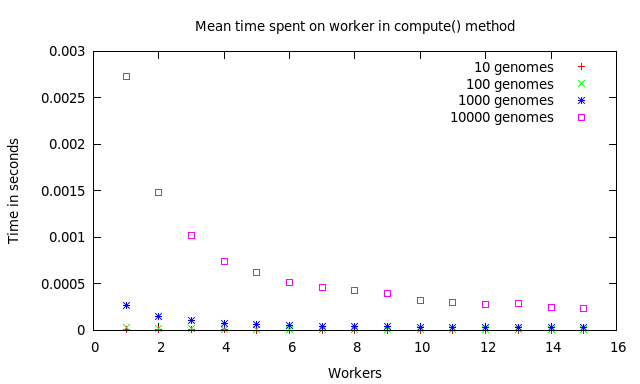
\includegraphics[width=100mm]{nsgaii-workertime.png}
%   \caption{ZDT-3 mean execution times spent on the workers \texttt{compute} method}
%   \label{fig:nsgaii-workertime}
% \end{figure}
% 
% The bad worker speedups for small genome sizes don't explain the bad algorithm speedups for bigger genome sizes, as the worker speedups for big genome sizes scale almost linearly. Figure \ref{fig:nsgaii-tasktime} helps to find a better suited explanation. It shows the mean time for the execution of a single task without the time spent in the workers \texttt{compute} method.
% 
% \begin{figure}
%   \centering
%   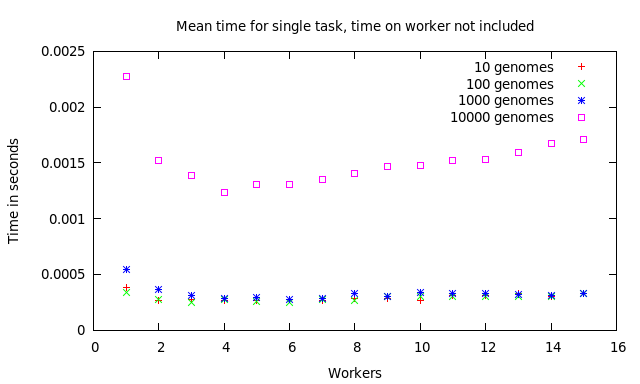
\includegraphics[width=100mm]{nsgaii-tasktime.png}
%   \caption{ZDT-3 mean execution times for a single task, without the time spent on the workers \texttt{compute} method}
%   \label{fig:nsgaii-tasktime}
% \end{figure}
% 
% One can see that the task time decreases for all benchmarks until two to four workers are used. Then it starts to increase. This behavior was not expected, rather it was expected that the task times keep decreasing as the number of workers increase because more tasks are executed in parallel.

The next step is to investigate the network performance. Calculations give a first hint to understand if the bad speedups can be explained with the saturation of the \unit[1]{Gb} network (a small ``b'' denotes bits, a big ``B'' denotes bytes, e.g., \unit[1]{Gb} = 1 gigabit, \unit[1]{GB} = 1 gigabyte). In each benchmark, 250 iterations on 100 individuals are performed, resulting in 25000 tasks. The tasks are send from the master to the workers and the workers return the results. The task data send from the master to the worker contains two individuals. Each individual consists of its genome, where each value in the genome is of type \texttt{double} (8 bytes). For a genome size of 10, this makes 2 (parents) $\times$ 10 (genomes) $\times$ 8 (bytes) $\times$ 25000 (tasks) = 4000000 bytes (\unit[4]{MB}) or \unit[32]{Mb} of data that needs to be transferred from the master to the workers during the benchmark. The size of the results sent from the workers to the master is about the half, as it consists of an individual (the offspring) and its fitness (the fitness is composed of two \texttt{double} values). This fact allows to use the outgoing data amount as upper bound for the network usage: if the outgoing data rate doesn't exceed the network bandwidth. This will be true also for the incoming data. Table \ref{table:network} shows the results for all genome sizes together with the best algorithm execution times. One can see from the table that the benchmark data can be transferred on the \unit[1]{Gb} Ethernet network during the according fastest algorithm execution time.

\begin{table}
  \centering
  \begin{tabular}{r|r|r|r}
    genomes & data [Mb] & \parbox[t]{3cm}{theoretical\\transfer time [s]} & \parbox[t]{3cm}{fastest algorithm\\execution time [s]}\\ \hline
    10 & 32 & 0.032 & 7.072 \\
    100 & 320 & 0.32 & 7.031 \\
    1000 & 3200 & 3.2 & 8.910 \\
    10000 & 32000 & 32 & 55.475 \\
  \end{tabular}
  \caption{Amount of network data sent from master to workers, theoretical transfer time and fastest algorithm execution}
  \label{table:network}
\end{table}

% The calculations are supported by observations of the network performance using the iftop utility \cite{iftop}. This tool shows, among other useful statistics, the peak network bandwidth for a given interface. The outgoing peak bandwidth on the Ethernet port of the master machine for a genome size of 10000 was about 400Mb/s. This is clearly below the theoretical limit of 1Gb/s for the used 1Gb Ethernet network.

% But 400Mb/s are to slow to transmit 32Gb data in 55 seconds, so how is it possible that a benchmark for 10000 genomes terminates after 55s? The explanation can be found once more in the YARN container placement. The 400Mb/s is the data rate that is send through the Ethernet port to the cluster, but worker containers that run on the same machine as the master don't use this port for communication. Instead, they communicate through the local interface. iftop showed an additional combined data transfer rate of 400Mb/s on the local interface when workers were running on the same machine as the master. This gives an aggregated peak data rate of 600 - 700Mb/s for the outgoing traffic, which is fast enough to transmit 32Gb of data in less than 55s.
 
% In cases where no workers executed on the same machine as the master the peak data rates on the Ethernet port and the algorithm execution times were higher. The results of three different tests with a genome size of 10000 were: 445Mb/s peak and 80s execution time, 426Mb/s peak and 86s execution time and 447Mb/s peak and 80s execution time. In all cases the execution time is sufficient to transfer the data from the master through the Ethernet to the workers. The peak data rates were in all cases below maximum network speed of 1Gb/s.

Additional experiments were performed to improve the confidence in the calculations and to establish the true achievable data rate for the network, given different message sizes. The experiments measure the peak network bandwidth using a small Java program and iftop.\footnote{\url{http://www.ex-parrot.com/pdw/iftop/} last access: 08.12.2014} The Java program uses the same communication techniques as Biohadoop (Netty + Kryo) and performs repeated request/response cycles between a master and several workers. The exchanged messages consist of 20, 200, 2000 or 20000 \texttt{double} values, corresponding to two parent individuals in the according ZDT-3 benchmarks. The resulting peak bandwidth was \unit[134]{Mb/s} for 20, \unit[489]{Mb/s} for 200, \unit[901]{Mb/s} for 2000 and \unit[552]{Mb/s} for 20000 \texttt{double} values. The CPU on the master was the limiting factor for 20, 200 and 20000 \texttt{double} values. For 2000 \texttt{double} values, the network was saturated at \unit[901]{Mb/s} and, therefore, the limiting factor. No studies were performed to explain why the experiments delivered the best results with 2000 values as this lies out of the scope of this thesis.

One phenomena regarding the network bandwidth needs further investigation. The above measurements show a peak data rate of \unit[552]{Mb/s} for the case of 20000 \texttt{double} values. If this data rate is taken as a basis for the ZDT-3 benchmark with 10000 genomes, one can calculate that more than \unit[55]{s} are needed to exchange \unit[32]{Gb} of data over the network between the master and its workers (\unit[32000]{Mb} / \unit[552]{Mb/s} = \unit[57.97]{s}). The explanation can be found once more in the YARN container placement. The \unit[552]{Mb/s} peak bandwidth is the data rate that is send through the Ethernet port to the cluster, but worker containers that run on the same machine as the master don't use this port for communication. Instead, they communicate through the local interface. iftop showed an additional combined data transfer rate of \unit[400]{Mb/s} (send and receive data rates are added) on the local interface when workers were running on the same machine as the master. This gives an aggregated peak data rate of \unit[700]{Mb/s} to \unit[800]{Mb/s} for the outgoing traffic, which is fast enough to transmit \unit[32]{Gb} of data in less than \unit[55]{s}. The execution times were higher in cases where no workers executed on the same machine as the master.

The calculations and additional experiments show that the network is fast enough to transfer the ZDT-3 benchmark data. The reason for the bad ZDT-3 speedups lie elsewhere.

This leads to the assumption that the benchmarks are CPU bound which was confirmed through observations of the CPU usage of the master. In the case of 10 and 100 genomes the CPU limit was reached by the master with two workers, for 1000 and 10000 genomes the limit was reached with four workers.

The high CPU utilization is caused by two effects: the first one is the object serialization/deserialization overhead that ranges between \unit[30]{\%} to \unit[40]{\%} for genome sizes of 10 and goes up to \unit[60]{\%} to \unit[70]{\%} for a genome size of 10000. Small genome sizes mean a high rate of both exchanged messages and serializations/deserializations. Large genome sizes reduce the rate of exchanged messages but increase the amount of work for a single serialization/deserialization.

The second effect is a direct consequence of computationally small worker tasks like in the case of 10 to 100 genomes: the master performs (beside the communication aspects) the algorithms for ranking and crowding distance. The workers return their results fast as the computation is not intense. Therefore, the master has to compute the ranking and crowding distance at short intervals. This results in a CPU utilization of about \unit[25]{\%} to \unit[30]{\%} only for this computations.

In conclusion, the ZDT-3 benchmarks are CPU bound by the master due to the small computational effort on the workers and the resulting fast exchange of many small messages. Increased genome sizes provide better speedup results, but are again limited by the CPU of the master, as they have higher demands for object serialization/deserialization. The performance of the \unit[1]{Gb} network and the available memory are sufficient to not slow down the ZDT-3 benchmarks.

\subsection{Tiled Matrix Multiplication}
The optimization goal of this benchmark was to find optimal tile sizes such that a matrix multiplication performs as fast as possible. The theoretical speedups for TMM promise better results (see table \ref{table:theoretical_speedup}) as matrix multiplications are compute intense and clearly dominate the algorithm execution time. Figure \ref{fig:tiledmul_250_100_128x128} and \ref{fig:tiledmul_250_100_256x256} show the execution times. One can see that the execution times decrease with the number of workers. This scales until 12 workers, after which the execution times remain constant or even increase slightly. The reason for this is that the cluster offers 12 CPU cores in total. When all cores are fully utilized, which happens with 12 workers, additional workers have to share CPU resources. This negatively impacts the execution times. So, TMM is CPU bound by the workers.

\begin{figure}
  \centering
  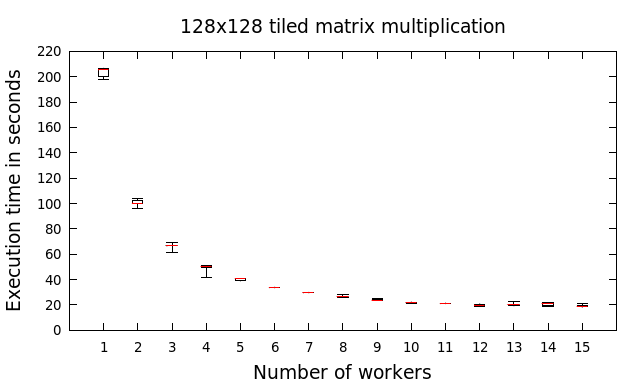
\includegraphics[width=100mm,natwidth=640,natheight=384]{tiledmul_250_100_128x128.png}
  \caption[TMM execution times for a matrix size of 128$\times$128]{TMM execution times for a matrix size of 128$\times$128}
  \label{fig:tiledmul_250_100_128x128}
\end{figure}
\begin{figure}
  \centering
  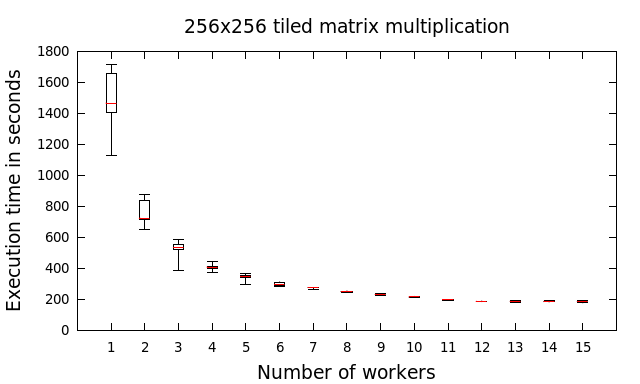
\includegraphics[width=100mm,natwidth=640,natheight=384]{tiledmul_250_100_256x256.png}
  \caption[TMM execution times for a matrix size of 256$\times$256]{TMM execution times for a matrix size of 256$\times$256}
  \label{fig:tiledmul_250_100_256x256}
\end{figure}

% The master is not as strongly demanded as in the ZDT-3 benchmarks, because the worker execution times are higher which results in less CPU stress on the master for object serialization/deserialization. Also, the master doesn't have to compute the ranking and crowding distance. 

An additional advantage of TMM benchmarks over the ZDT-3 benchmarks is the small amount of data that needs to be transmitted. Like in the ZDT-3 benchmarks, each task data consists of two parents that are sent from the master to the worker, the result is an offspring with its fitness value. In contrast to ZDT-3 --- where an individual consists of a number of \texttt{double} values according to its genome size --- a TMM individual consists of the tile sizes for the $i$, $j$ and $k$ loop. Each of them is a single \texttt{integer} with 4 bytes. The total amount of data that needs to be transmitted from the master to the workers is therefore $2 \times 3 \times 4 \times 25000 = 600000$ bytes or \unit[4.8]{Mb}. Together with the computationally intense tasks of matrix multiplication on the workers (leading to lower network usage) and the absence of time consuming ranking and crowding distance algorithms on the master, this provides speedups of up to 10.507 for 128$\times$128 matrices and 7.961 for 256$\times$256 matrices.

The reason for the better performance of the 128$\times$128 benchmark over the 256$\times$256 benchmark is unknown. A possible explanation is that the tile sizes are taken from a bigger range (256 instead of 128) which makes it more likely that bad tile sizes are chosen. This is, however, pure speculation.

% The results show less scattering in contrast to ZDT-3. This is due to the fact, that the matrix multiplications dominate the execution times. The location of the YARN containers and the time needed for the communication between the master and its workers have therefore a smaller impact on the execution times. Only the five benchmarks for \ref{fig:tiledmul_250_100_256x256} with one worker shows an elevated amount of scattering. The reason is unknown, as the master and the worker were located on different machines in all benchmarks with this settings. 

\subsection{Speedups}
Figure \ref{fig:speedup} depicts the speedups for all test problems with respect to increasing worker sizes. The ZDT-3 benchmarks show poor results. This is not surprising as the maximum theoretical speedups of this problem are small (see table \ref{table:theoretical_speedup}) and the communication overhead is bigger compared to TMM. The only unexpected outcome was that the benchmarks scale very bad with a maximum speedup of 2.498 for 1000 genomes. The reason is that the ZDT-3 benchmarks are CPU bound by the master, as the investigations in section \ref{chap:evaluation:result:zdt3} suggest.

TMM demonstrate better results, the maximum speedup was 10.507 for a matrix size of 128$\times$128. In this case, the speedup grows near linear or even slightly better than linear with the number of workers. That a speedup is better than linear is usually suspicious but can be explained by the fact that each benchmark was repeated five times and the average times of this five executions were taken to compute the speedups. Five executions seem to be too small for getting smooth results, especially when taking into account that the YARN container placement has big influences on the execution times.

The speedups for the 128$\times$128 TMM increase until a worker size of 12 is reached. At this point, no more improvements are achieved. The reason for this is the limited number of CPUs in the cluster.

The speedup for the 256$\times$256 TMM benchmark is worse compared to the 128$\times$128 TMM, although it also grows nearly linear until 12 workers.

\begin{figure}
  \centering
  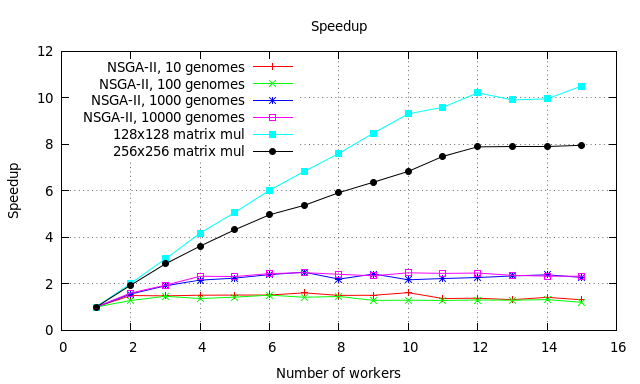
\includegraphics[width=130mm,natwidth=640,natheight=384]{speedup.png}
  \caption[Speedups for ZDT-3 and TMMs]{Speedups for ZDT-3 and TMMs}
  \label{fig:speedup}
\end{figure}

% 
% 
% Each physical machine in the cluster provides two cores, the master reaches its theoretical limit when it uses 200\% of the CPU resources, which means that both CPU are fully utilized by the master. The practical CPU limit is at about 150\%, because other processes run at the same time on the same machine. This limit is further reduced if worker containers are executed at the same time on the same machine. 
% 
% As each physical machine in the cluster provides two cores, the master reaches its theoretical limit when it uses 200\% of the CPU resources, which means that both CPU are fully utilized by the master. The practical CPU limit is at about 150\%, because other processes run at the same time on the same machine. This limit is further reduced if worker containers are executed at the same time on the same machine. 


% The ZDT-3 benchmarks show that the speedup does not scale well with the number of workers. The reason for this is that the time spent by the worker on offspring creation and fitness evaluation is only a small fraction of the time it takes to complete a task. For a genome size of 10 and one worker, this fraction is for example 2.124\% and reduces to 0.596\% for 15 workers. For a genome size of 100 the fraction ranges from 8.765\% for one worker to 1.138\% for 15 worker. For a genome size of 1000 it ranges from 33.100\% to 7.044\% and for a genome size of 10000 it ranges from 54.556\% to 11.789\%. So the ZDT-3 benchmark is clearly bound by the communication between the master and its workers. This explains also the overall poor scaling when workers are  added.
% 
% The execution time results for ZDT-3 are shown in figure \ref{fig:nsga_250_100_10}, \ref{fig:nsga_250_100_100}, \ref{fig:nsga_250_100_1000} and \ref{fig:nsga_250_100_10000}. One thing to notice is that the benchmark results for given settings are distributed in a broad range, e.g. they range from 9.637s to 14.164s for ZDT-3 with a genome size of 100 and one worker (see figure \ref{fig:nsga_250_100_100}).
% 
% % \begin{figure}
% %   \centering
% %   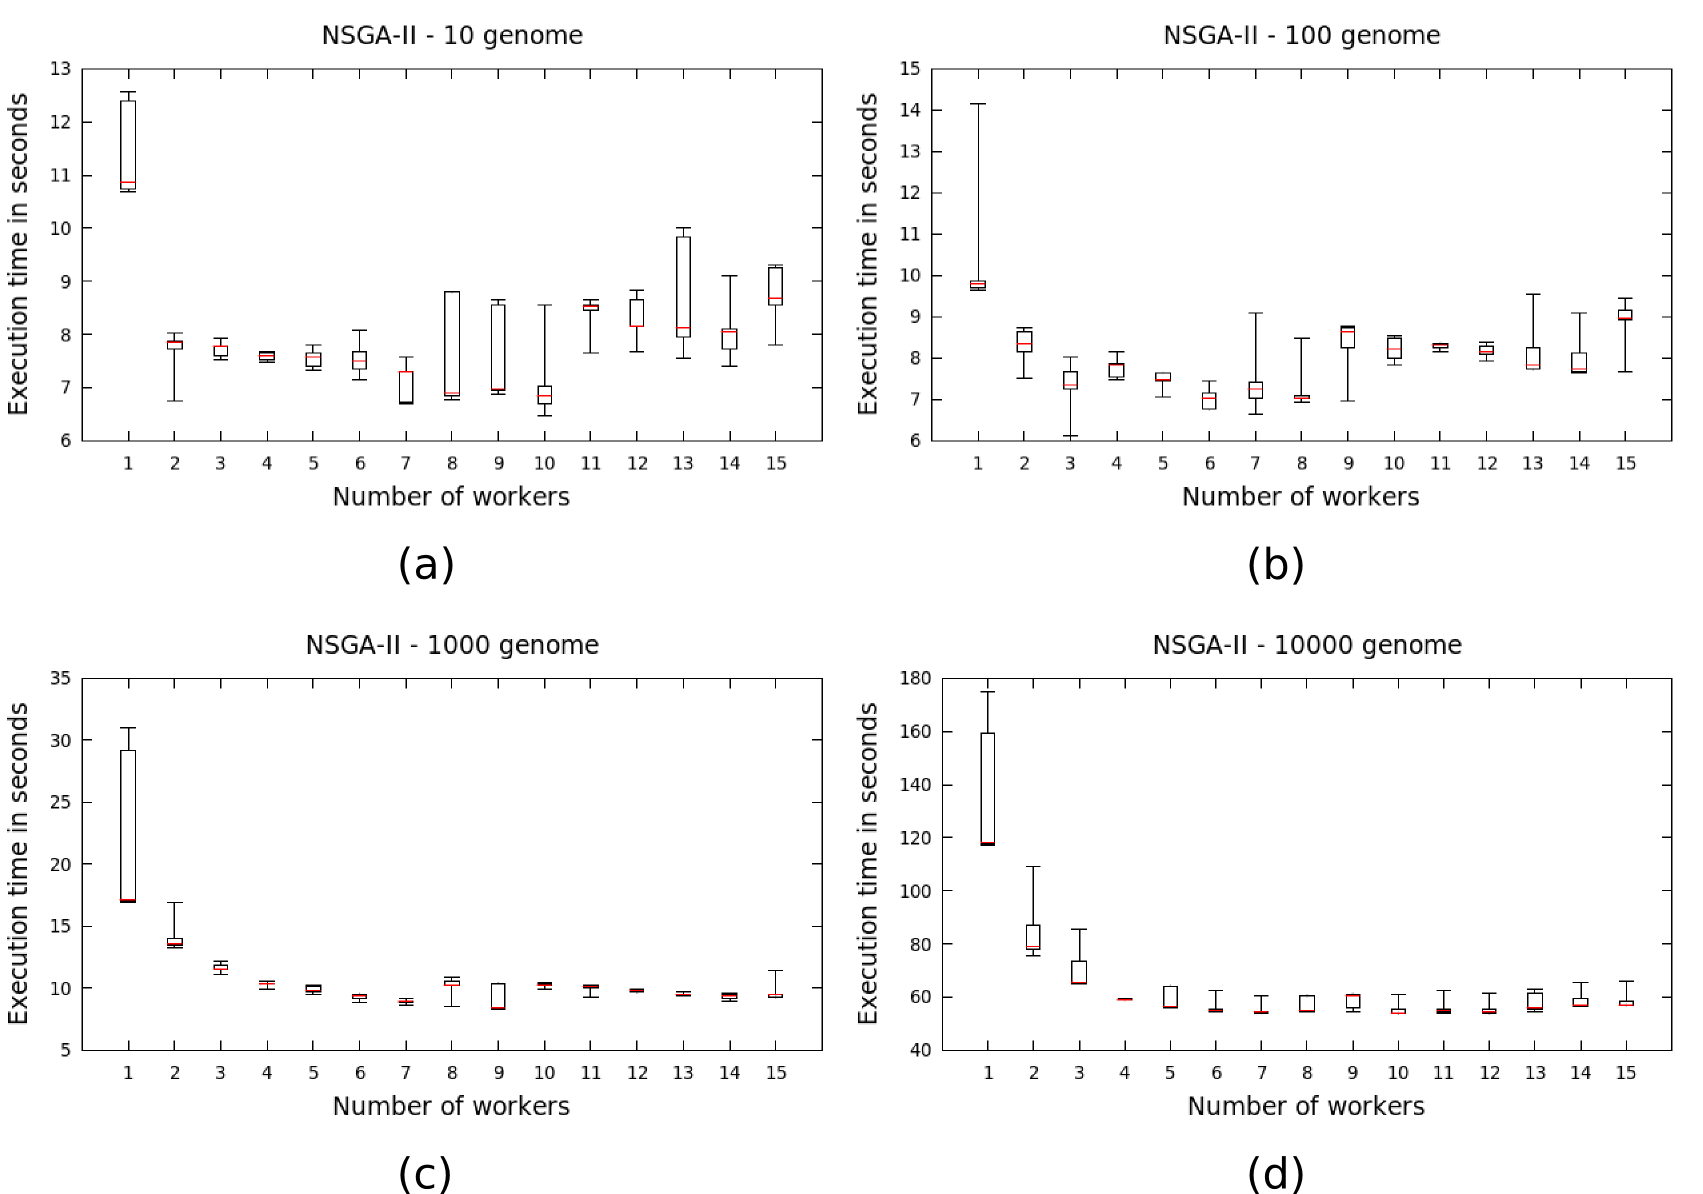
\includegraphics[width=130mm]{nsgaii_250_100.png}
% %   \caption{ZDT-3 execution times. All benchmarks were performed with 250 iterations and a population size of 100. (a) genome size=10, (b) genome size=100, (c) genome size=1000, (d) genome size=10000}
% %   \label{fig:nsga_250_100}
% % \end{figure}
% 
% 
% 
% The reason for this is the location of the YARN containers in the cluster while a benchmark runs. Figure \ref{fig:nsga_250_100_100} is used as example: for the benchmark with one worker, 4 out of 5 benchmarks executed with both the master and worker container running on the same machine, resulting in better performance. A worker that is located on the same machine as the master can communicate to the master without using a physical network, which reduces the communication time. During the fifth benchmark, the master and worker were executed on different containers. The 4 benchmarks with master and worker on the same machine took 9,761s on average, the benchmark where master and worker were located on different machines took 14.164s to execute.
% 
% The same explanation applies to the other benchmarks with 1 to 6 workers in figure \ref{fig:nsga_250_100_10} to \ref{fig:nsga_250_100_10000}, except for the benchmark for one worker in figure \ref{fig:nsga_250_100_10}. This deviation is not due of container placement, the scattered results are the result of other factors that couldn't be established.
% 
% The container placement is done automatically by YARN and can not be influenced, without modifying the YARN environment - which was not done for this thesis. The placement can have advantages like in the example above, but can also negatively impact the performance.
% 
% As an example, look at the benchmark for 8 workers in figure \ref{fig:nsga_250_100_10}. For two benchmarks, YARN placed the master and two worker containers on the same machine. As each machine has only two cores, this worsens the execution time results. The master container has to share its CPU resources with two other containers, that have already a high resource demand. This slows the master down and with it the whole application. The numbers for this example are 6.842s (on average) for the benchmarks where the master had to share its machine with only one worker. In the case the master were placed together with two other containers on the same machine the execution time was on average 8.799s.
% 
% The more the cluster is utilized, the more it is likely that more than two containers execute on the same machine. This can be particularly seen in figures \ref{fig:nsga_250_100_10} and \ref{fig:nsga_250_100_100} for the benchmarks with six and more workers.
% 
% Figure \ref{fig:nsga_250_100_1000} and \ref{fig:nsga_250_100_10000} show a similar but less pronounced behavior for more than six workers, as they are less communication bound than the previous examples. Both figures show a high dependency on the container placement for a small number of workers, e.g. for one worker.
% 
% Figure \ref{fig:nsga_250_100_10} shows that more than two workers have no significant impact on the execution time for a genome size of 10. The execution time remains almost the same when workers are added. The reason for this is the bad work time to task time ratio mentioned above. Figure \ref{fig:nsga_250_100_100} shows advantages for up to 9 workers for a genome size of 100 - if the container placement comes in favor. More workers increase the execution time. Figure \ref{fig:nsga_250_100_1000} shows also advantages for up to 9 workers for a genome size of 1000. The scattering is reduced in most of the figures benchmark, compared to the previous benchmarks. Figure \ref{fig:nsga_250_100_10000} shows the results for a genome size of 10000. The best results are obtained between 6 to 12 workers, more workers increase the execution time. The speedup properties for this benchmark are better compared to the previous ones, as the work time to task time ratio is way better.

% The theoretical speedups for TMM show better results (see table \ref{table:theoretical_speedup}), as matrix multiplications are compute intense and clearly dominate the algorithm execution time. Figure \ref{fig:tiledmul_250_100_128x128} and \ref{fig:tiledmul_250_100_256x256} shows the execution times for TMM test problem. The execution times for a matrix size of 128x128 are given in figure \ref{fig:tiledmul_250_100_128x128}. One can see that the execution time decreases with the number of workers. This scales until 12 workers, after which the execution time remains the same or slightly increases. The reason for this is, that the cluster offers 12 CPU cores in total. When all cores are fully utilized, which happens with 12 workers, additional workers have to share CPU cores. This negatively impacts the execution times. The same observations are true for figure \ref{fig:tiledmul_250_100_256x256}.
% 
% The results show less scattering in contrast to ZDT-3. This is due to the fact, that the matrix multiplications dominate the execution times. The location of the YARN containers and the time needed for the communication between the master and its workers have therefore a smaller impact on the execution times. Only the five benchmarks for \ref{fig:tiledmul_250_100_256x256} with one worker shows an elevated amount of scattering. The reason is unknown, as the master and the worker were located on different machines in all benchmarks with this settings. 
% 
% \begin{figure}
%   \centering
%   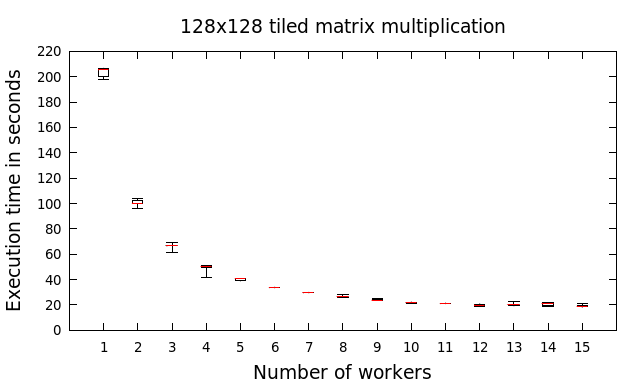
\includegraphics[width=100mm]{tiledmul_250_100_128x128.png}
%   \caption{TMM execution times. All benchmarks were performed with 250 iterations and a population size of 100. (a) matrix size=128x128, (b) matrix size=256x256}
%   \label{fig:tiledmul_250_100_128x128}
% \end{figure}
% \begin{figure}
%   \centering
%   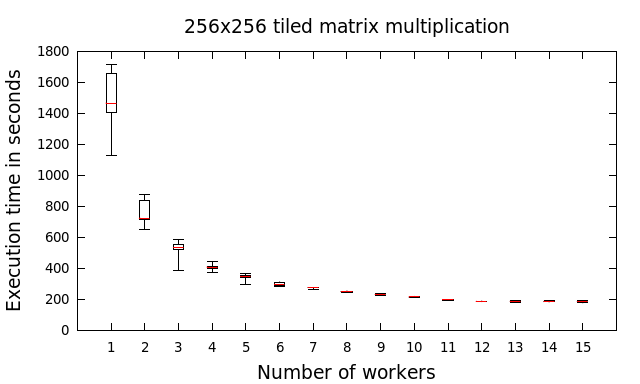
\includegraphics[width=100mm]{tiledmul_250_100_256x256.png}
%   \caption{TMM execution times. All benchmarks were performed with 250 iterations and a population size of 100. (a) matrix size=128x128, (b) matrix size=256x256}
%   \label{fig:tiledmul_250_100_256x256}
% \end{figure}
% 
% Figure \ref{fig:speedup} shows the speedups for all test problems with respect to increasing worker sizes. TMM shows good results. In the case of 128x128 TMM, the speedup grows near linear or even slightly better with the number of workers. That a speedup is better than linear was not expected but can be explained by the fact that each benchmark was repeated 5 five times, which seems to be to small to get smooth results. After 6 workers, the 128x128 benchmark shows good speedups until a worker size of 12 is reached. At this point, no more improvements are achieved, the reason for this is the number of CPUs in the cluster. The speedup for the 256x256 TMM benchmark is worse compared to the 128x128 TMM, although it grows nearly linear until 12 workers.
% 
% The speedups for the ZDT-3 benchmarks are not so good. Specially small genome sizes deliver poor results with speedups of less than 2 for genome sizes of 10 and 100, no matter how many workers are used. Increasing the genome size provides better results, using 1000 genomes provides a speedup of 2.498 using 7 workers. A genome size of 10000 provides a maximum speedup of 2.479 using 8 workers. Overall, the ZDT-3 benchmarks show only small improvements when workers are added, increasing the number of workers beyond 8 to 10 doesn't provide any benefit. This is not surprising as the maximum theoretical speedups of this problems are small (see table \ref{table:theoretical_speedup}) and the communication overhead is bigger compared to TMM.
% 
% \begin{figure}
%   \centering
%   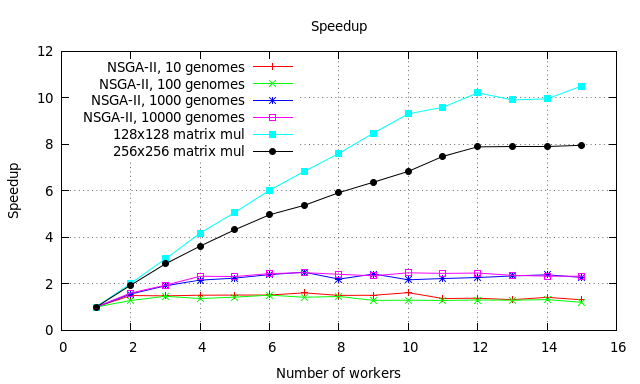
\includegraphics[width=130mm]{speedup.png}
%   \caption{Speedup for ZDT-3 and TMM}
%   \label{fig:speedup}
% \end{figure}
% 
% Another observation was, that the number of worker containers running on the same machine as the master could affected the execution times negatively.